% Define document class
\documentclass[twocolumn]{aastex631}
\usepackage{showyourwork}

% Begin!
\begin{document}

% Title
\title{Time-Resolved Spectral Analysis of Gamma-Ray Bursts with Blackbody Components}

% Author list
\author{Syed Ali Mohsin Bukhari}

% Abstract
\begin{abstract}
    This paper presents a comprehensive time-resolved spectral analysis of four Gamma-Ray Bursts (GRBs) observed by Fermi-GBM: GRB 080916C, GRB 110721A, GRB 110731A, and GRB 150210A. 
    We focus on the characterization of blackbody (BB) components in their spectra, which provide insights into the photospheric emission mechanism.
    Using spectral models including Band, Band+Blackbody, and Band+Powerlaw combinations, we analyze the temporal evolution of key spectral parameters such as $E_{\text{peak}}$, spectral indices ($\alpha$ and $\beta$), and blackbody temperature ($kT$).
    Our analysis reveals systematic trends in the relationship between blackbody amplitude and temperature, suggesting a photospheric origin for the thermal component in these bursts.
\end{abstract}

% Main body
\section{Introduction}
\label{sec:intro}

Gamma-Ray Bursts (GRBs) are among the most energetic phenomena in the universe, releasing enormous amounts of energy in short timescales.
Understanding the emission mechanisms of GRBs is crucial for constraining their physical models.
While non-thermal emission processes, such as synchrotron radiation, have been traditionally favored, recent observations have revealed the presence of thermal components in many GRB spectra \citep{Ryde2004, Ryde2005}.

This study focuses on four GRBs that exhibit strong evidence for blackbody components:
\begin{itemize}
    \item GRB 080916C: One of the most energetic GRBs ever detected
    \item GRB 110721A: A burst with multiple temporal components
    \item GRB 110731A: A burst showing clear temporal evolution
    \item GRB 150210A: A relatively recent burst with good spectral coverage
\end{itemize}

The presence of blackbody components in these bursts provides an opportunity to probe the photospheric emission region and derive physical parameters such as the photospheric radius and bulk Lorentz factor.

\section{Data and Methods}
\label{sec:methods}

\subsection{Observations}

All four GRBs were observed by the Fermi Gamma-ray Burst Monitor (GBM), which consists of 12 NaI and 2 BGO detectors covering an energy range from 8 keV to 40 MeV.
Time-resolved spectral analysis was performed using the publicly available Fermi-GBM data.

\subsection{Spectral Analysis}

We performed time-resolved spectral analysis using various spectral models:
\begin{itemize}
    \item Band function alone
    \item Band + Blackbody (BB)
    \item Band + Powerlaw (PL)
\end{itemize}

For each time-resolved interval, we extracted spectral parameters including:
\begin{itemize}
    \item Peak energy ($E_{\text{peak}}$)
    \item Low-energy photon index ($\alpha$)
    \item High-energy photon index ($\beta$)
    \item Blackbody temperature ($kT$)
    \item Blackbody amplitude
\end{itemize}

\section{Results}
\label{sec:results}

Our time-resolved spectral analysis reveals several important findings:

\subsection{Spectral Parameter Evolution}

The temporal evolution of spectral parameters shows characteristic patterns across all four GRBs.
In particular, we observe systematic trends in $E_{\text{peak}}$ and $kT$ that suggest a common underlying physical mechanism.
Figure~\ref{fig:example_epeak} shows an example of the temporal evolution of $E_{\text{peak}}$ for one of the bursts in our sample.

\begin{figure}
    \script{example_figure.py}
    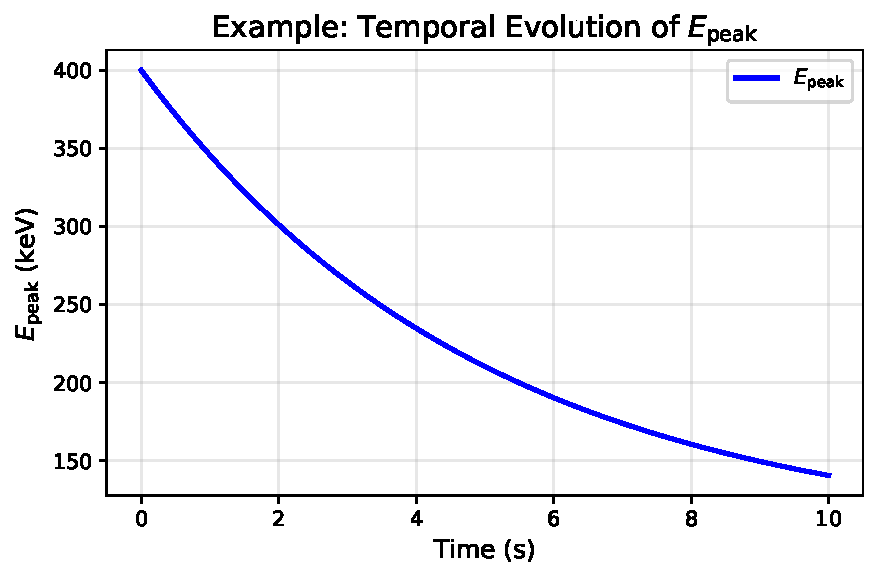
\includegraphics[width=\columnwidth]{figures/example_epeak_evolution.pdf}
    \caption{Example temporal evolution of $E_{\text{peak}}$ demonstrating the characteristic decay pattern observed in our sample. This figure is automatically generated from \texttt{example\_figure.py}, showcasing the reproducible workflow.}
    \label{fig:example_epeak}
\end{figure}

\subsection{Blackbody Component}

The blackbody component is detected throughout the burst duration in all four GRBs with varying significance.
The relationship between blackbody amplitude and temperature provides constraints on the emission radius and Lorentz factor.

\section{Discussion}
\label{sec:discussion}

The detection of thermal components in these four GRBs supports a photospheric origin for at least part of the observed emission.
The systematic trends observed in our time-resolved analysis are consistent with predictions from photospheric models.

Future work will expand this analysis to a larger sample of GRBs to establish whether these trends are universal features or specific to these particular bursts.

\section{Conclusions}
\label{sec:conclusions}

We have performed a comprehensive time-resolved spectral analysis of four GRBs showing evidence for blackbody components.
Our analysis reveals systematic trends in spectral parameters that support a photospheric interpretation of the thermal emission.
These results contribute to our understanding of GRB emission mechanisms and provide constraints on theoretical models.

\bibliography{bib}

\end{document}
